\documentclass[12pt]{article}
\usepackage[margin=1in]{geometry}
\usepackage{natbib}
\usepackage{graphicx}
\usepackage{subcaption}
\bibliographystyle{apalike}
\begin{document}

\title{Peachy}
%\author{Dianne Velasco, Malli Aradhya, Jeffrey Ross-Ibarra}
\author{
 \small\sfbf{Shohei Takuno$^{\ast ,1}$, Peter Ralph$^{\dag, \ddag}$, Kelly Swarts$^{\S}$, Rob J. Elshire$^{\S}$, Jeffrey C. Glaubitz$^{\S}$,}\\
   \small\sfbf{Edward S. Buckler$^{\S, \ast\ast}$, Matthew B. Hufford$^{\ast, \dag\dag}$, and Jeffrey Ross-Ibarra$^{\ast,\ddag\ddag,}$}\thanks{
Corresponding author:  Department of Plant Sciences, University of California, Davis, California 95616, USA. 
    E-mail: \mbox{rossibarra@ucdavis.edu}}\\[0.3cm]
   \small\sf $^{\ast}$Department of Plant Sciences, University of California, Davis, California 95616, USA,\\
   \small\sf $^\dag$Department of Evolution and Ecology, University of California, Davis, California 95616, USA,\\
   \small\sf $^\ddag$Molecular and Computational Biology, University of Southern California,  Los Angeles,California 90089-0371, USA,\\
   \small\sf $^\S$Institute for Genomic Diversity, Cornell University, Ithaca, New York 14853-2703, USA,\\
   \small\sf $^{\ast\ast}$United States Department of Agriculture Agricultural Research Service, Ithaca,
NY 14853, USA,\\
   \small\sf $^{\dag\dag}$Department of Ecology, Evolution, and Organismal Biology, Iowa State University, Ames, Iowa 50011, USA,\\
   \small\sf $^{\ddag\ddag}$The Center for Population Biology and the Genome Center, University of California, Davis, California 95616 , USA,\\
   \small\sf $^1$ Present address: SOKENDAI (Graduate university for advanced studies), Hayama, Kanagawa 240-0193, Japan
}

\maketitle

\section*{Introduction}
Dianne is awesome.

\section*{Methods}
Millions of peaches, peaches for me.

\subsection*{Samples}
Peaches come from a can, where they were put there by a man in a factory downtown.

Thinking about population demography and effects on genetic architecture of traits.

intro to quantitative traits

 understanding them is key

 traditionally, QTL has been used

 recently GWAS, potential to identify individual genes

 missing heritability

rare alleles of large negative effect often missed \citep{Thornton2013}


demographic effects (figure \ref{fig:pairwise}) can impact deleterious allele distro

$V_a$ influenced by demography \citep{Lohmueller2014}


These guys did crap \citep{Gazave2013}.
But \citet{Thornton2014} did more.


\begin{figure}[b]
\centering
   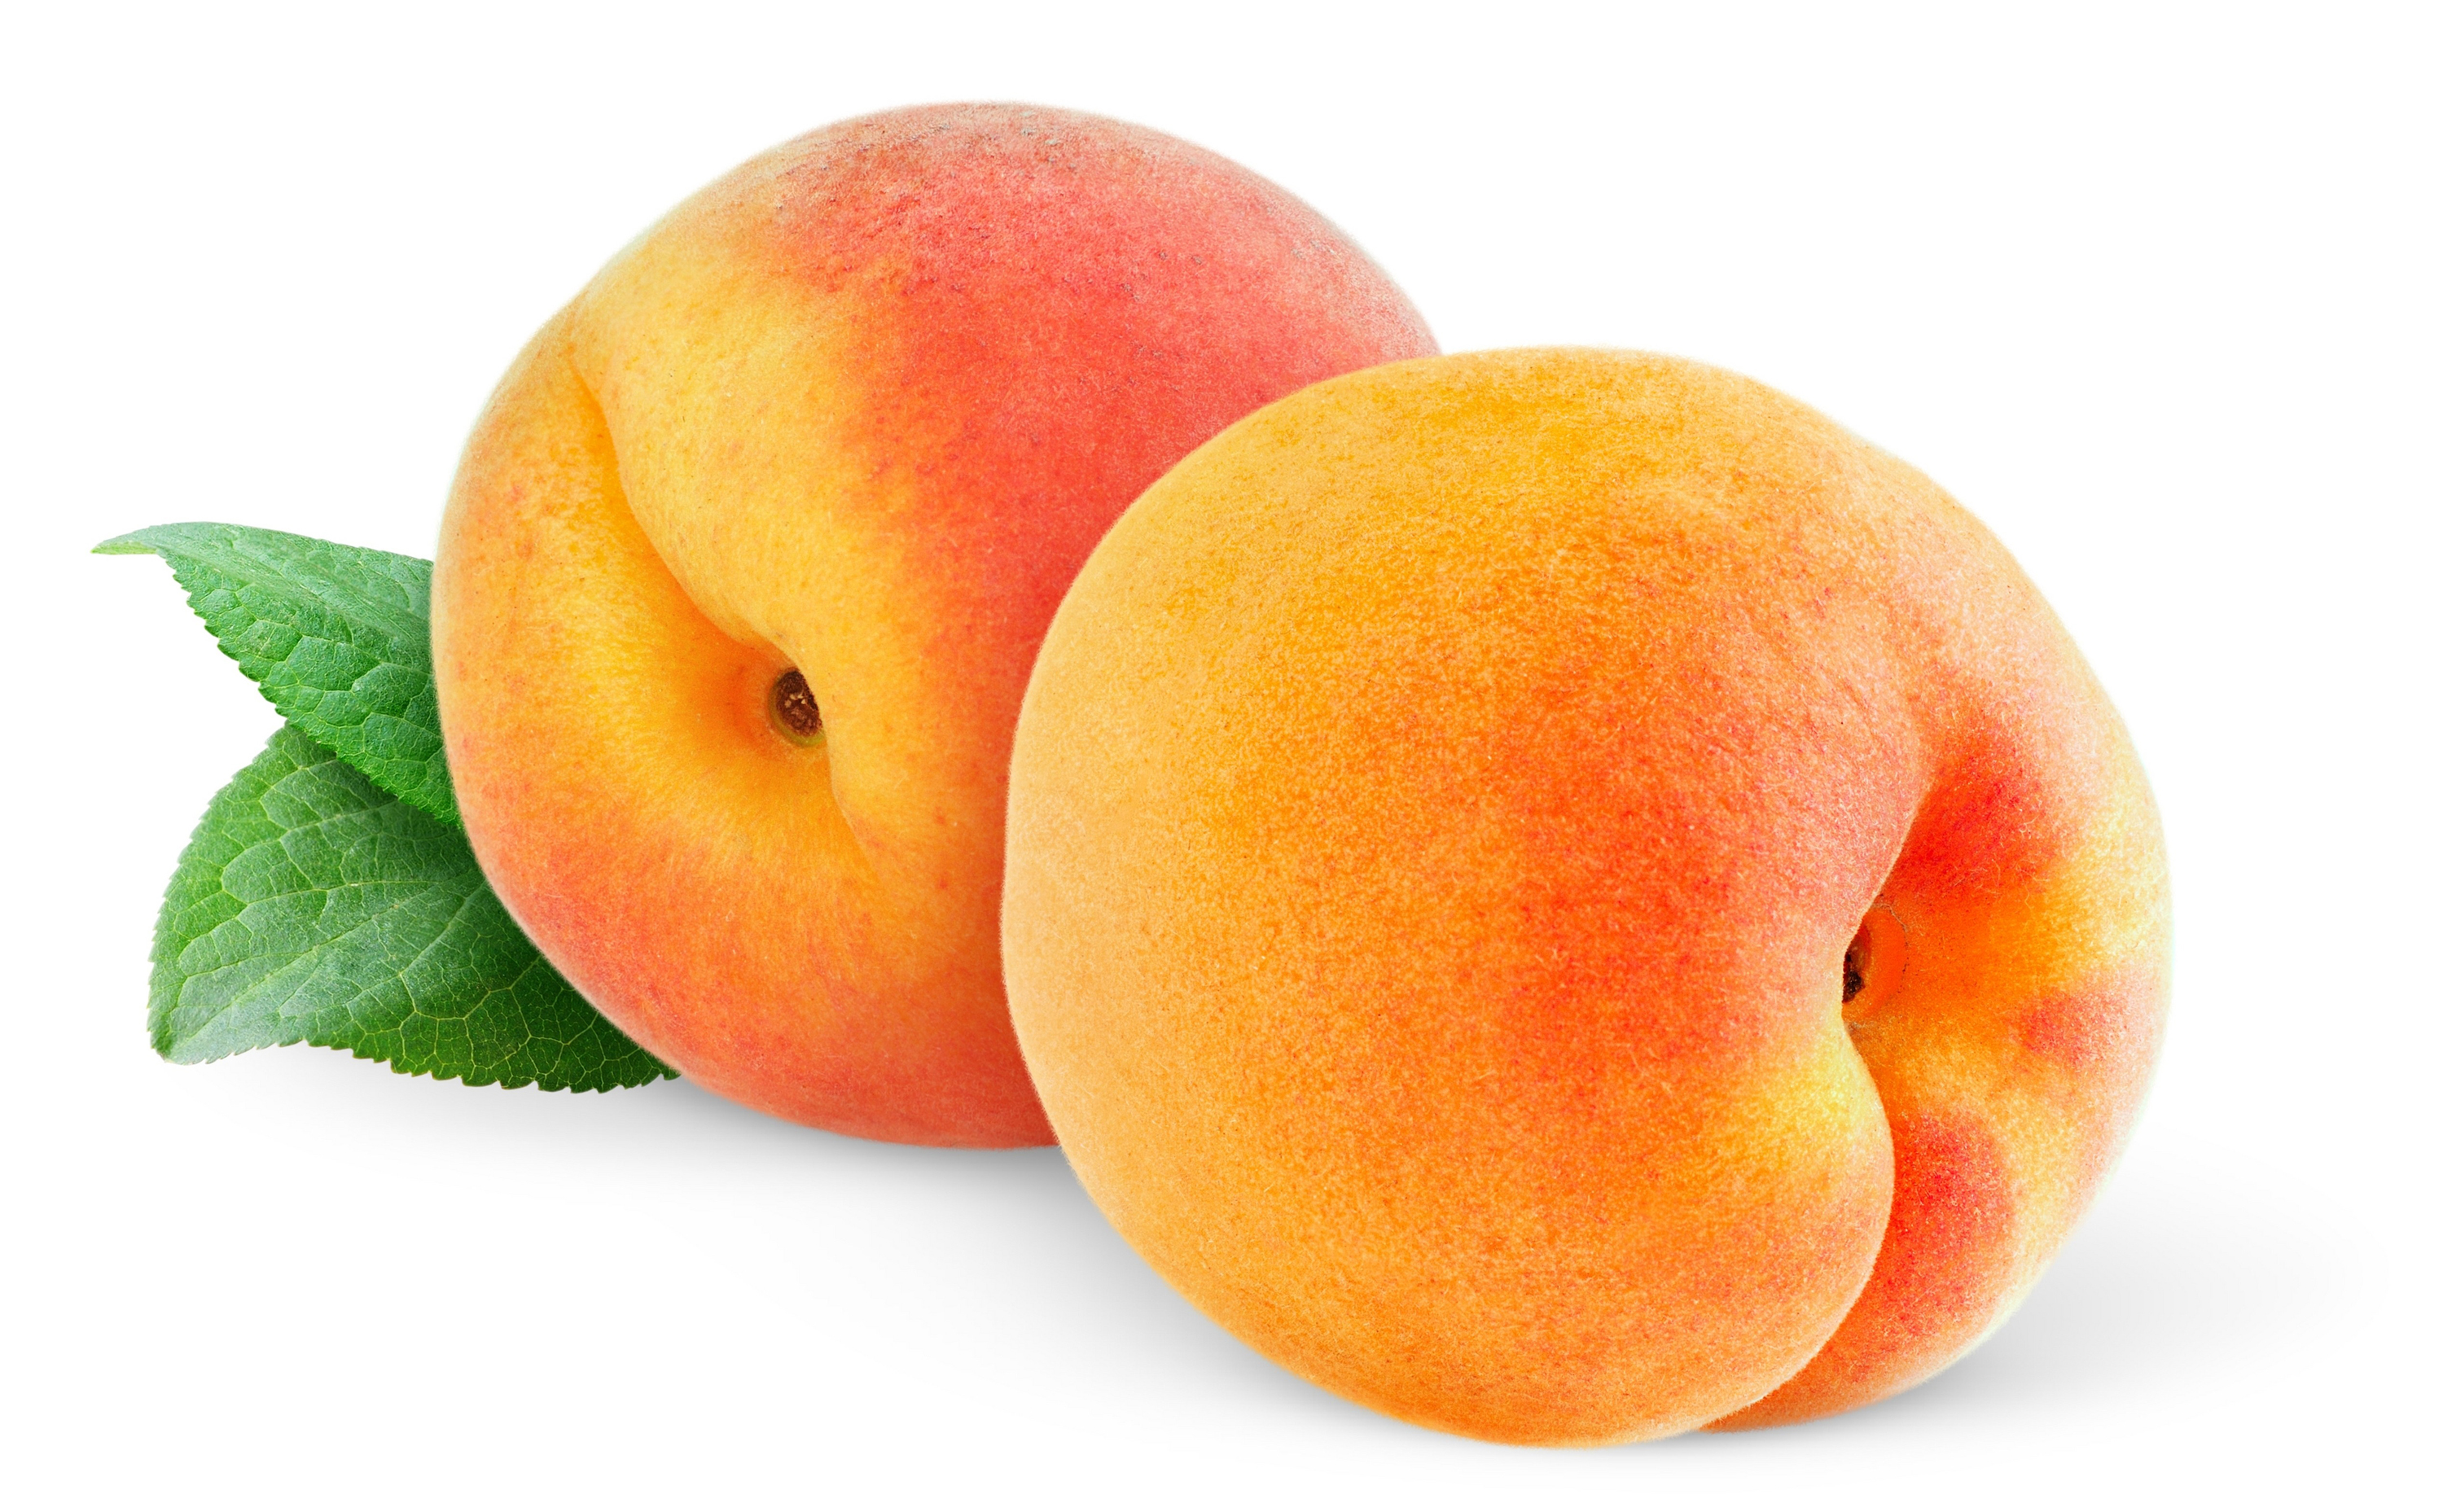
\includegraphics[width=0.8\textwidth]{peachzdfgad.jpg}
  \caption{All polymorphisms}
  \label{fig:pairwise}
\end{figure}%


For designing breeding strategies, for utilizing diversity from wild relatives, for understanding variation in phenotype, for engineering new traits (GMOs, CRISPR).




\bibliography{/Users/jri/Documents/references/references.bib}
\end{document}